% Global
\documentclass[parskip=full,a4paper]{scrartcl}
\usepackage{blindtext}
\usepackage[utf8]{inputenc}
\usepackage{etoolbox}

% Graphics
\usepackage{pdfpages}
\usepackage{graphicx}

% Layout
\usepackage[margin=1in]{geometry}
\usepackage{setspace}
\setstretch{1.3}

% Inline-code
\usepackage[outputdir=./_build]{minted}
\setminted{fontsize=\scriptsize,baselinestretch=0}

% Bibliography
\usepackage{natbib}
\usepackage{bibentry}
\nobibliography*

% Title
\title{nETL}
\author{Zach Smith}
\date{\today}
 
 % Document
\begin{document}

% Title page
\maketitle
\tableofcontents
\newpage

% Test figures and tables
\begin{figure}
    \caption{Dummy figure}
\end{figure}
\begin{table}
    \caption{Dummy table}
\end{table}

% Content
\section{Abstract}

Hello world 2
\section{Introduction}

This is the first section.

Lorem  ipsum  dolor  sit  amet,  consectetuer  adipiscing
elit.   Etiam  lobortisfacilisis sem.  Nullam nec mi et
neque pharetra sollicitudin.  Praesent imperdietmi nec ante.
Donec ullamcorper, felis non sodales...

\section{Code Snippet}

This is a code snippet:

\begin{minted}{javascript}
    (function() {
        console.log('hi');
    })();
\end{minted}

\section{citation example}

This is a citation \cite{bower16}.

\begin{figure}[h]
    \centering
    % \includepdf[pages={1},scale=0.7,pagecommand=\chapter]{../resources/figures/netlUML.pdf}
    \includegraphics[scale=0.4]{./resources/figures/netlUML.pdf}
    \caption{Description of figure}
\end{figure}

\newpage

% Appendix
\begin{appendix}
    \listoffigures
    \listoftables
\end{appendix}
\newpage

% Bibliogrpahy
\bibliographystyle{plain}
\bibliography{../bibliography/msc_citations.bib}

% Close docuemnt
\end{document}